\documentclass[addpoints,12pt]{exam}
\usepackage[utf8]{inputenc}
\usepackage[spanish,es-noshorthands]{babel}
\usepackage{amsmath,amssymb}
\usepackage{graphicx}
\usepackage{array}
\usepackage{xcolor}
\usepackage{tikz}
\usetikzlibrary{calc,arrows.meta}
\usepackage[most]{tcolorbox}
\usepackage[legalpaper,margin=2cm,top=1.8cm]{geometry}

\graphicspath{{./}}
\definecolor{ubbblue}{RGB}{0,51,102}
\definecolor{wireblue}{RGB}{20,50,170}

\qformat{}
\newcommand{\qpts}[1]{{\setlength{\fboxsep}{2.5pt}\fbox{#1}}\hspace{0.6em}\ignorespaces}
\newcommand{\qhead}[1]{\thequestion.\hspace{0.5em}\qpts{#1}}
\newcommand{\pts}[1]{\textcolor{red}{\textbf{(#1 pts)}}}

% simbolos de corriente: sale (punto) y entra (cruz)
\newcommand{\isale}[1]{%
  \draw[ubbblue,line width=1.4pt,fill=white] (#1) circle (0.2);
  \fill[ubbblue] (#1) circle (0.075);}
\newcommand{\ientra}[1]{%
  \draw[ubbblue,line width=1.4pt,fill=white] (#1) circle (0.2);
  \draw[ubbblue,line width=1.4pt] ($(#1)+(-0.13,-0.13)$)--($(#1)+(0.13,0.13)$)
        ($(#1)+(-0.13,0.13)$)--($(#1)+(0.13,-0.13)$);}

\pagestyle{headandfoot}
\runningheadrule
\firstpageheader{}{}{}
\runningheader{\small F\'isica II - Electromagnetismo}%
              {\small\textbf{Certamen 4 -- Forma A}}%
              {\small 27 de Noviembre, 2026}
\firstpagefooter{}{\thepage}{}
\runningfooter{}{Page \thepage\ of \numpages}{}

\begin{document}

%========================================================
% PORTADA
%========================================================
\begin{center}
    
\includegraphics[height=1.9cm]{logo ubb.png}\hspace{1cm}%
    
\includegraphics[height=1.5cm]{logo dfis.png}\\[0.5cm]
    {\Large F\'isica II - Electromagnetismo}\\[0.15cm]
    {\LARGE\textbf{Certamen 4}}\\[0.2cm]{\Large Forma A}\\[0.9cm]
    27 de Noviembre, 2026
\end{center}

\vspace{0.7cm}

\noindent\textbf{Nombre Completo}: \hrulefill\\[0.7cm]
\noindent\textbf{Rut}: \makebox[6.5cm]{\hrulefill}\hspace{0.3cm}\textbf{Carrera}: \hrulefill

\vspace{0.4cm}
\noindent\rule{\textwidth}{1pt}
\vspace{0.2cm}

\noindent\textbf{Algunas consideraciones para esta evaluaci\'on:}
\begin{itemize}\setlength\itemsep{2pt}
    \item El certamen 4 contiene \numpages\ p\'aginas (incluida la portada) y \numquestions\ preguntas,
          con un total de \numpoints\ puntos.
    \item Cada pregunta debe ser respondida por s\'olo una respuesta. En caso de presentar m\'as de
          una, se anulan las respuestas.
    \item \textbf{No est\'a permitido el uso de celulares o tablet en el desarrollo de esta
          evaluaci\'on. De ser sorprendido utilizando estos art\'iculos su evaluaci\'on ser\'a
          calificada con nota 1.0.}
    \item Buena suerte!
\end{itemize}

\noindent Seleccione con una \textbf{X} el nombre del profesor de su secci\'on:

\vspace{0.15cm}
\noindent
\begin{minipage}{0.49\textwidth}
\begin{tabular}{|l|p{1.1cm}|}
\hline
Prof.\ Diego Ram\'irez & \\ \hline
Prof.\ Mor\'in \'Ordenes & \\ \hline
Prof.\ Luis Liempi & \\ \hline
Prof.\ Luis Soto & \\ \hline
\end{tabular}
\end{minipage}%
\begin{minipage}{0.49\textwidth}
\begin{tabular}{|l|p{1.1cm}|}
\hline
Prof.\ Ismael C\'aceres & \\ \hline
Prof.\ Evelyn Riveros & \\ \hline
Prof.\ Arturo Fern\'andez & \\ \hline
~ & \\ \hline
\end{tabular}
\end{minipage}

\vspace{0.9cm}
\begin{center}
{\large\textbf{Puntaje}}\\[0.2cm]
\gradetable[v][questions]
\end{center}

\newpage

%========================================================
% PREGUNTAS
%========================================================
\begin{questions}

%--------------------------------------------------------
% PREGUNTA 1  (Biot-Savart - forma A)
%--------------------------------------------------------
\question[20]
\begin{minipage}[t]{0.52\textwidth}
\vspace{0pt}
\qhead{20}Una corriente $I = 100$ [mA] viaja por el alambre de la Fig.~1 desde el punto $(+)$
hasta el punto $(-)$. El alambre est\'a formado por un arco de radio menor $R_1 = 10{,}0$ [cm], un
tramo recto y un arco de radio mayor $R_2 = 20{,}0$ [cm], ambos arcos centrados en el origen.
Usando la ley de Biot-Savart, calcule el campo magn\'etico en el origen del sistema coordenado
generado por dicha corriente.
\end{minipage}\hfill
\begin{minipage}[t]{0.44\textwidth}
\vspace{0pt}
\centering
\begin{tikzpicture}[scale=1.15, >=Stealth, line width=0.9pt]
    \draw[->] (-2.5,0)--(2.4,0) node[right]{$X$};
    \draw[->] (0,-2.5)--(0,2.6) node[above]{$Y$};
    \draw[wireblue,line width=2.2pt] (-45:1) arc[start angle=-45, end angle=90, radius=1];
    \draw[wireblue,line width=2.2pt] (0,1)--(0,2);
    \draw[wireblue,line width=2.2pt] (90:2) arc[start angle=90, end angle=270, radius=2];
    \draw[line width=0.6pt] (0,0)--(-45:1);
    \draw[line width=0.6pt] (0.42,0) arc[start angle=0, end angle=-45, radius=0.42];
    \node[font=\small] at (1.45,-0.62){$45^\circ$};
    \node[font=\large] at ($(-45:1)+(0.22,-0.2)$){$+$};
    \node[font=\large] at (0.25,-2.15){$-$};
    % radios
    \draw[->,line width=0.7pt] (0,0)--(30:1);
    \node[font=\small,above left=-1pt] at (30:0.62){$R_1$};
    \draw[->,line width=0.7pt] (0,0)--(150:2);
    \node[font=\small,above right=-1pt] at (150:1.15){$R_2$};
\end{tikzpicture}
\\[2pt]
{\footnotesize Fig.\ 1.}
\end{minipage}

\medskip
\noindent\textbf{(a)} Determine el campo magn\'etico en el origen producido por el arco de radio
menor $R_1$. \pts{7}

\vspace{7.5cm}
\noindent\textbf{(b)} Determine el campo magn\'etico en el origen producido por el arco de radio
mayor $R_2$. \pts{7}

\vspace{7.5cm}
\noindent\textbf{(c)} Determine el campo magn\'etico en el origen producido por el tramo recto.
\pts{3}

\vspace{3.5cm}
\noindent\textbf{(d)} Determine el campo magn\'etico total en el origen. \pts{3}

\newpage

%--------------------------------------------------------
% PREGUNTA 2  (fuerza entre conductores)
%--------------------------------------------------------
\question[20]
\begin{minipage}[t]{0.56\textwidth}
\vspace{0pt}
\qhead{20}La Fig.~2 muestra
tres conductores rectil\'ineos infinitos, perpendiculares al plano de la hoja, por los que circulan
las corrientes $I_1 = 10$ [A], $I_2 = 30$ [A] e $I_3 = 20$ [A], respectivamente, en los sentidos indicados.

\smallskip
\noindent\textbf{Nota.} El sentido positivo del eje $z$ sale de la hoja. Las unidades est\'an en
metros. S\'imbolos: $\odot$ sale de la hoja ($+z$); $\otimes$ entra en la hoja ($-z$).
\end{minipage}\hfill
\begin{minipage}[t]{0.40\textwidth}
\vspace{0pt}
\centering
\begin{tikzpicture}[scale=1.0, >=Stealth, line width=0.9pt]
    \draw[->] (-0.8,0)--(3.4,0) node[right]{$+x$};
    \draw[->] (0,-0.6)--(0,3.4) node[above]{$+y$};
    \isale{0,0}
    \ientra{2.6,0}
    \isale{0,2.6}
    \node[ubbblue,above left] at (-0.12,0.12){$I_2$};
    \node[ubbblue,above] at (2.6,0.25){$I_1$};
    \node[below] at (2.6,-0.25){$0{,}2$};
    \node[ubbblue,right] at (0.25,2.6){$I_3$};
    \node[left] at (-0.25,2.6){$0{,}2$};
\end{tikzpicture}
\\[2pt]
{\footnotesize Fig.\ 2.}
\end{minipage}

\medskip
\noindent Determine:

\smallskip
\noindent\textbf{(a)} La fuerza magn\'etica por unidad de longitud que ejerce el conductor 1 sobre el
conductor 3. \pts{8}

\vspace{6.5cm}
\noindent\textbf{(b)} La fuerza magn\'etica por unidad de longitud que ejerce el conductor 2 sobre el
conductor 3. \pts{8}

\vspace{6.5cm}
\noindent\textbf{(c)} La fuerza magn\'etica resultante por unidad de longitud sobre el conductor 3.
\pts{2}

\vspace{2.5cm}
\noindent\textbf{(d)} Dibuje el vector de la fuerza resultante por unidad de longitud con origen en el
centro de la secci\'on transversal del conductor 3. \pts{2}

\newpage

%--------------------------------------------------------
% PREGUNTA 3  (induccion)
%--------------------------------------------------------
\question[19]
\qhead{19}Considere un solenoide de radio $r = 5$ [cm] con $n = 400$ [vueltas/metro] por el que
circula una corriente dada por $I(t) = \tfrac{1}{6}\,e^{-3t}$ [A]. Fuera del solenoide, pero
conc\'entrica a \'el, se encuentra una bobina de radio $2r$ con $N = 20$ espiras, que tiene una
resistencia el\'ectrica $R_e = 20$ [$\Omega$]. En las figuras se muestran el corte transversal y el
corte longitudinal del sistema. Calcule:

\begin{center}
\begin{minipage}[c]{0.35\textwidth}
\centering
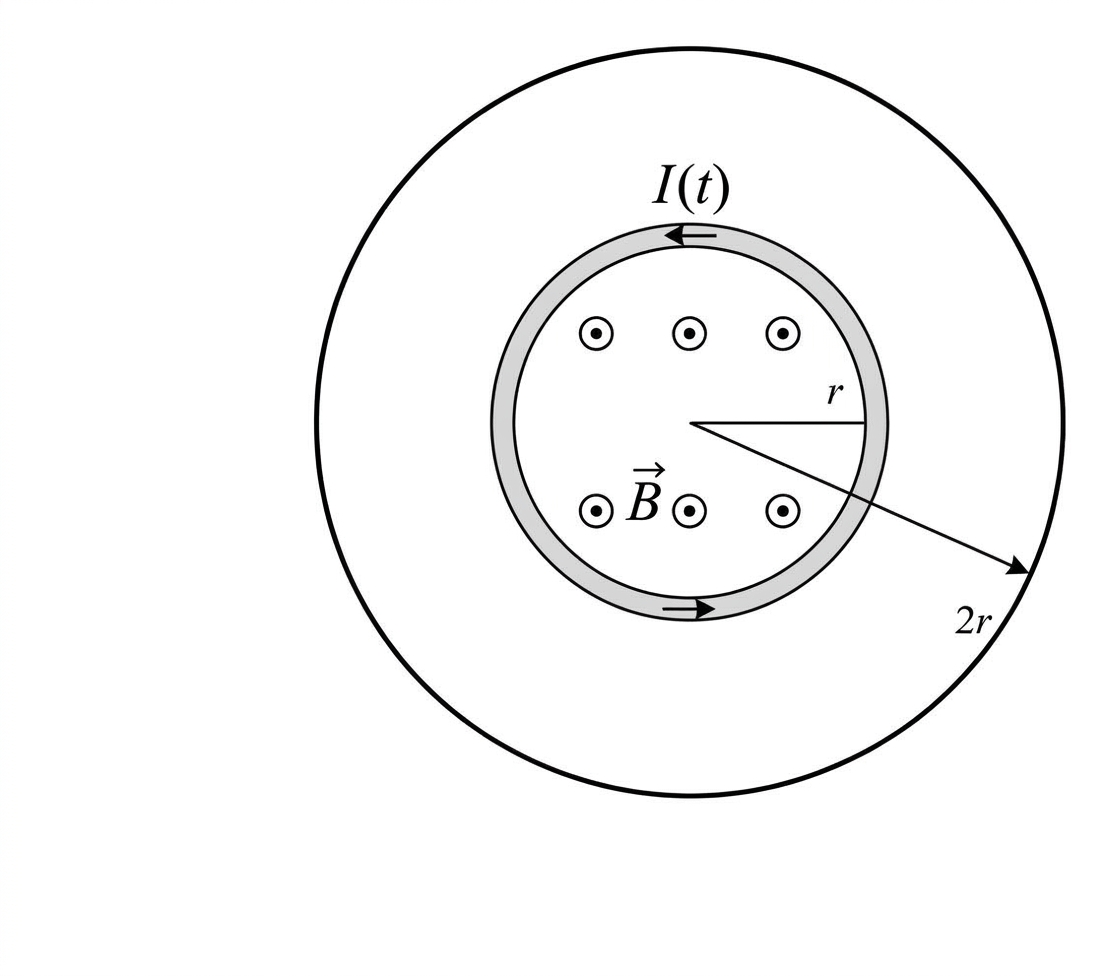
\includegraphics[width=\textwidth]{bobinas-vista-aerea.jpg}\\[2pt]
{\footnotesize Fig.\ 3a. Corte transversal.}
\end{minipage}\hfill
\begin{minipage}[c]{0.58\textwidth}
\centering
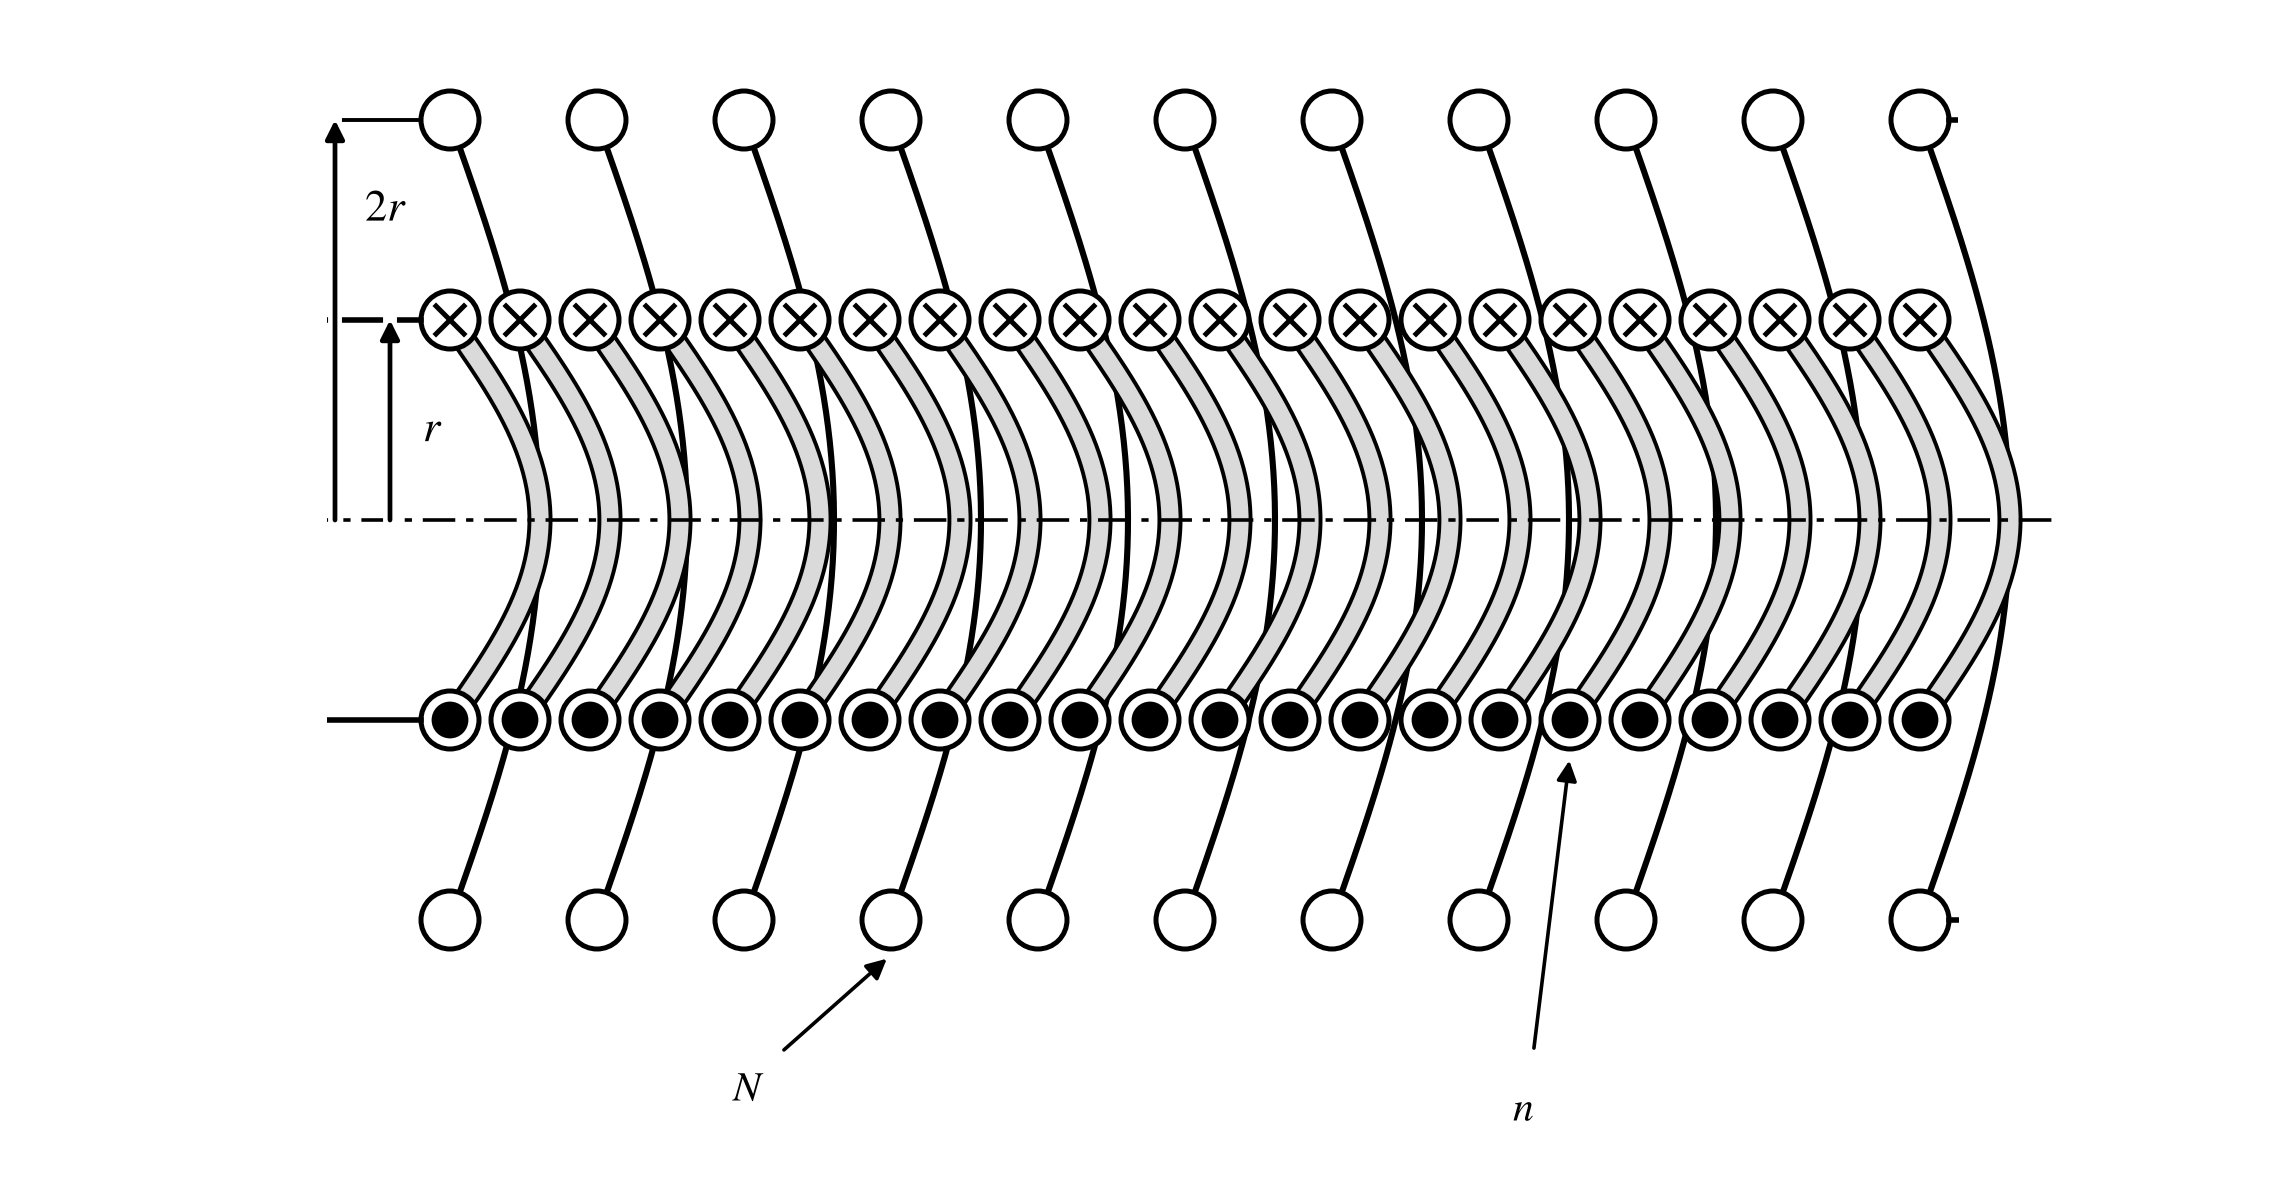
\includegraphics[width=\textwidth]{corte_longitudinal_bobinas_bn.png}\\[2pt]
{\footnotesize Fig.\ 3b. Corte longitudinal.}
\end{minipage}
\end{center}
\medskip
\noindent\textbf{(a)} El flujo magn\'etico $\Phi_B$ a trav\'es de la bobina. \pts{7}

\vspace{5.5cm}
\noindent\textbf{(b)} La fem inducida en la bobina. \pts{6}

\vspace{4.5cm}
\noindent\textbf{(c)} La corriente inducida en la bobina. Adem\'as, de acuerdo a la ley de Lenz,
indique si la direcci\'on del campo magn\'etico inducido es la \textbf{misma} o
\textbf{diferente} a la del campo magn\'etico del solenoide. Justifique. \pts{6}

\end{questions}

\newpage

%========================================================
% FORMULARIO
%========================================================
\newtcolorbox{formbox}[1]{colback=gray!3, colframe=gray!55, coltitle=black,
    colbacktitle=white, fonttitle=\bfseries, boxrule=0.5pt, arc=2pt,
    left=6pt,right=6pt,top=2pt,bottom=2pt, before skip=4pt, after skip=4pt,
    title={#1}}
\setlength{\jot}{2pt}

\begin{center}{\large\textbf{Formulario}}\end{center}
\vspace{-0.1cm}

\begin{formbox}{Ley de Biot-Savart}
\[
    d\vec{B}=\frac{\mu_0 I}{4\pi}\,\frac{d\vec{\ell}\times(\vec{r}-\vec{r}\,')}{|\vec{r}-\vec{r}\,'|^{3}}
    \ ;\qquad
    dB=\frac{\mu_0 I}{4\pi}\,\frac{d\ell\,\sin\theta}{|\vec{r}-\vec{r}\,'|^{2}}
\]
\end{formbox}

\begin{formbox}{Ley de Amp\`ere}
\[
    \oint\vec{B}\cdot d\vec{\ell}=\mu_0\,I_{\text{enc}}
\]
\end{formbox}

\begin{formbox}{Fuerza magn\'etica sobre una corriente}
\[
    \vec{F}=I\,\vec{L}\times\vec{B}
\]
\end{formbox}

\begin{formbox}{Flujo magn\'etico}
\[
    \Phi_B=\int_S\vec{B}\cdot d\vec{S}
\]
\end{formbox}

\begin{formbox}{Ley de Faraday-Lenz y ley de Ohm}
\[
    \varepsilon=-N\,\frac{d\Phi_B}{dt}\ ;\qquad \varepsilon=i\,R
\]
\end{formbox}

\begin{formbox}{Productos cruz de los vectores unitarios}
\centering
$\hat{\imath}\times\hat{\jmath}=\hat{k}$,\quad
$\hat{\jmath}\times\hat{k}=\hat{\imath}$,\quad
$\hat{k}\times\hat{\imath}=\hat{\jmath}$,\qquad
$\hat{\imath}\times\hat{\imath}=\hat{\jmath}\times\hat{\jmath}=\hat{k}\times\hat{k}=\vec{0}$
\end{formbox}

\begin{formbox}{Constantes y prefijos}
$\mu_0=4\pi\times10^{-7}$ [T$\cdot$m/A]. \qquad
$c=10^{-2}$, \quad $m=10^{-3}$, \quad $\mu=10^{-6}$, \quad $n=10^{-9}$.
\end{formbox}

\end{document}
